\documentclass{beamer}
\usetheme{metropolis}

\setbeamertemplate{bibliography item}[text]

\usepackage{amsmath}
\usepackage{amsfonts}
\usepackage{graphicx}
\usepackage{setspace}
\usepackage{braket}
\usepackage{float}
\usepackage{tikz}


\makeatletter
\newcommand\mathcircled[1]{%
  \mathpalette\@mathcircled{#1}%
}
\newcommand\@mathcircled[2]{%
  \tikz[baseline=(math.base), color=red] \node[draw,circle,inner sep=1pt] (math) {$\m@th#1#2$};%
}
\makeatother

\title{Quantum Bogosort}
\subtitle{Chicago STEM Fair, Design}
\date{March 18, 2022}
\author{George Huebner (Grade 12), Michael Caines (Teacher Sponsor)}
\institute{Walter Payton College Prep}
\begin{document}
  \maketitle
  
  % we looove red tape
  \begin{frame}[plain, noframenumbering]{Attachments}
    \begin{columns}
        \column{0.5\textwidth}
            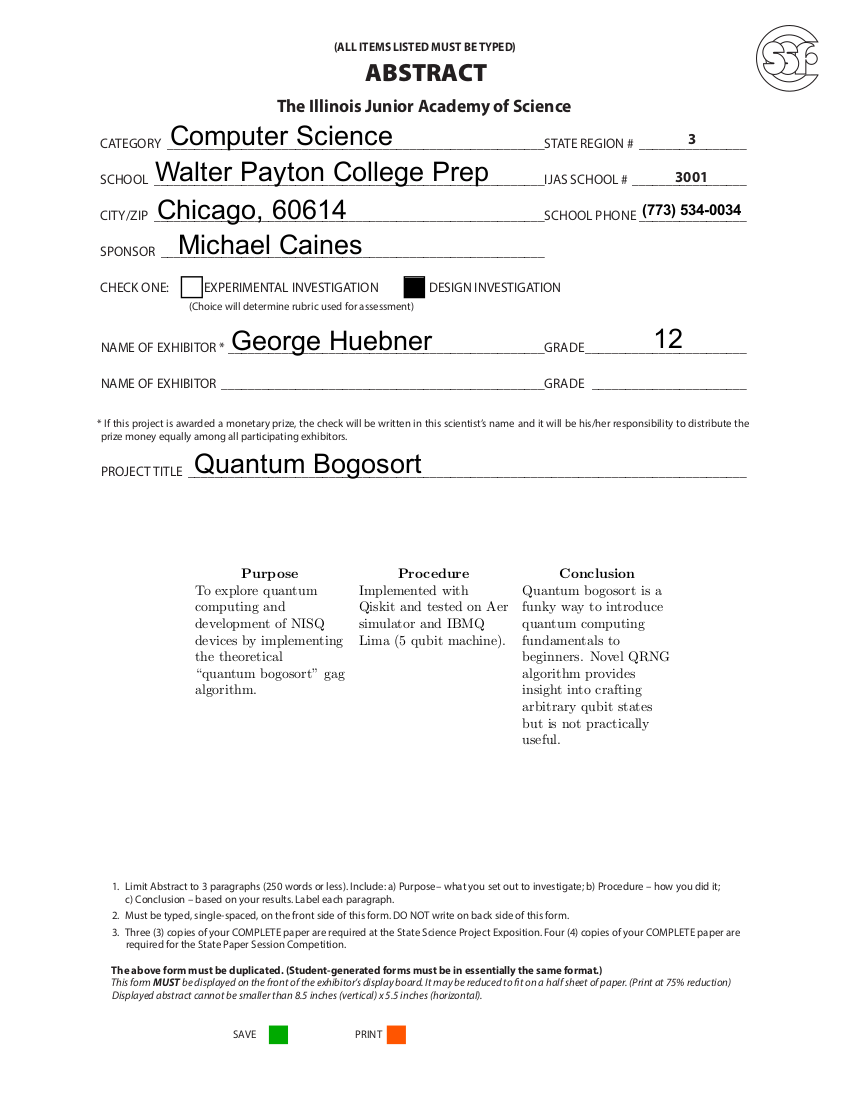
\includegraphics[width=\linewidth]{images/abstract.png}
        \column{0.5\textwidth}
            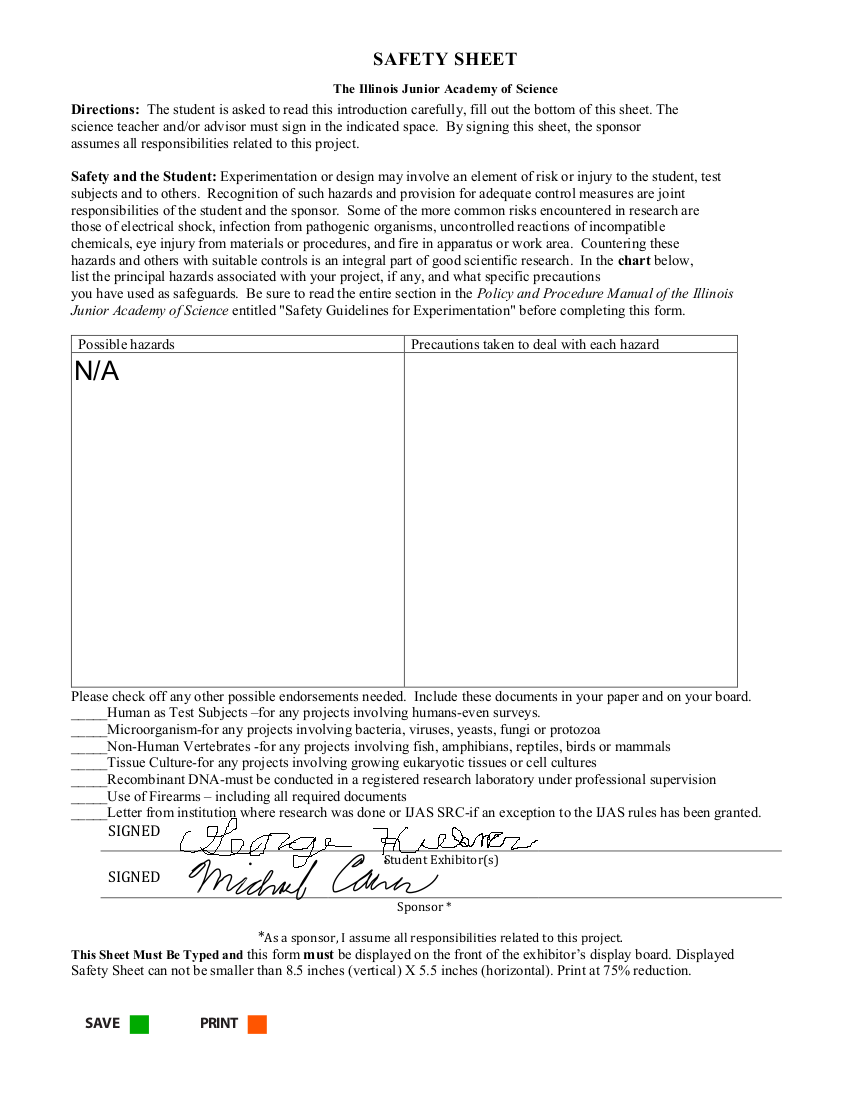
\includegraphics[width=\linewidth]{images/safety_sheet.png}
    \end{columns}
  \end{frame}
  
  \section{Introduction}
  
  \begin{frame}{Abstract}
    Gag algorithms are a staple of computer science and provide many a good chuckle. Take, for instance, MiracleSort\textsuperscript{\color{blue}\cite{thompson_2013}}, an algorithm that relies on alpha particle emission to cause erroneous bit flips to sort the list:
    \begin{center} \texttt{while isSorted(unsorted\_list) is False: \\ \hspace{-70} time.sleep(1000)} \end{center}
    Despite their apparent uselessness, joke algorithms provide valuable insight into algorithm design and complexity\textsuperscript{\color{blue}\cite{gruber_holzer_ruepp_2007}}. In this paper we propose an implementation to Quantum Bogosort, one such joke algorithm.
  \end{frame}
  
  \begin{frame}{What is Quantum Bogosort?}
    \textit{Classical} Bogosort is a sorting algorithm.
    \begin{enumerate}
        \item Randomly permute the list.
        \item If the list is sorted, done! Otherwise go to step 1.
    \end{enumerate}
    This has unbounded worst-case time complexity and an expected time complexity of $O(n \cdot n!)$. \\
    \vspace{10}
    \textit{Quantum} Bogosort is very similar to classical Bogosort, except it uses a quantum computer to permute the list.
  \end{frame}
  
  \begin{frame}{Attachments}
  Code + Paper: \href{https://github.com/Borris-the-real-OG/Quantum_Bogosort}{\color{blue} \underline{github.com/Borris-the-real-OG/Quantum\_Bogosort}}
  \end{frame}
  
  \begin{frame}{Acknowledgements}
  \begin{itemize}
  \item \href{https://qiskit.org/}{\color{blue} \underline{Qiskit}}
  \item \emph{We acknowledge the use of IBM Quantum services for this work. The views expressed are those of the authors, and do not reflect the official policy or position of IBM or the IBM Quantum team.\textsuperscript{\color{blue}\cite{ibm_21}}}
  \item All code was written and tested with Qiskit 0.32.0 \& Python 3.8 on WSL2 Ubuntu 20.04.1.
  \item Special thanks to Joe Clapis
  \end{itemize}
  \end{frame}
  
  \begin{frame}{Purpose}
  Just like its classical counterpart, Quantum Bogosort is pretty useless. In fact, classical sorting algorithms have been proven to have a lower bound time complexity of $ \Omega (N \log_2 N) $: there's nothing to optimize! \\
  \textbf{\textit{However}}, QBS presents a good case study for quantum algorithms; we present an analysis of implementation and complexity of QBS in a similar vein to Gruber et al.'s\textsuperscript{\color{blue}\cite{gruber_holzer_ruepp_2007}} analysis of classic bogosort.
  \end{frame}
  
  \section{Algorithm Design}
  
  \begin{frame}{QRNG}
    \begin{columns}[T,onlytextwidth]
        \column{0.48\textwidth}
            \vspace{20}
            Desired State: \\
            $$ \sum_{x=0}^{N-1} \frac{1}{\sqrt{N}} \ket{x_{BE}} $$
            This is quite easy to do with powers of 2; we just need to use Hadamard gates with control qubits to chunk a big number into smaller subproblems.
       \column{0.48\textwidth}
           \begin{align*}
                & \ket{\psi} = \mathcircled{\color{black} \frac{1}{\sqrt{2}}} \ket{0000} + \frac{1}{\sqrt{2}} \ket{1000} \\
                & \mathbf{CH(\psi_0, \psi_{[1, 3]}), \ X(\psi_0)} \\
                & \ket{\psi} = \mathcircled{\color{black} \frac{1}{\sqrt{16}}}(\ket{0000} + \ket{0001} + \\ 
                & ... + \ket{0111}) + \frac{1}{\sqrt{2}} \ket{1000}
            \end{align*}
            \color{red} We mostly care about amplitude as opposed to register state
    \end{columns}
  \end{frame}
  
  \begin{frame}{QRNG}
    \textbf{Limitation:} Hadamard gates create the state $ \frac{1}{\sqrt{2}} \ket{0} + \frac{1}{\sqrt{2}} \ket{1} $. What about states that aren't powers of 2? \\ \\
    \textbf{Solution:} Arbitrary rotation gates allow for qubit superposition with arbitrary amplitudes. \\
    Hadamard is just a rotation of $ \frac{\pi}{2} $ around the Pauli Y-axis!
    \begin{align*}
        &\ket{\psi} = \ket{0} \\
        & \text{R}_{\text{y}}(\theta) \ket{\psi} = \begin{bmatrix} \cos \frac{\theta}{2} & -\sin \frac{\theta}{2} \\ \sin \frac{\theta}{2} & \cos \frac{\theta}{2} \end{bmatrix} \ket{\psi} = -\sin \frac{\theta}{2} \ket{0} + \cos \frac{\theta}{2} \ket{1}
    \end{align*}
    \textit{Everything in this project is measured in Pauli-Z basis, so we don't worry about phase or imaginary numbers.}
  \end{frame}
  
  \begin{frame}{Algorithm}
  \begin{enumerate}
      \item If `parts' $= 2^\texttt{len(register)}$, use the control register to apply multi-controlled Hadamard gates to the rest of the register. Done.
      \item If `parts' $\leq 2^\texttt{len(register)}-1$, add \texttt{register[0]} to the control register and skip to step 5.
      \item Calculate $\theta$, R\textsubscript{y}$(\theta)$ the first register qubit, and add it to the control register.
      \item Using the control register, apply multi-controlled Hadamard gates to the rest of the register.
      \item Recurse on the remaining qubits. \\
  \end{enumerate}
  \end{frame}
  
  \begin{frame}{Worked Example}
    \begin{columns}
        \column{0.5\textwidth}
        $$i = 77, \ \ket{\psi} = \ket{0000000}$$
        \column{0.5\textwidth}
        $$\theta_0 = 2\arccos \sqrt{\frac{77-\color{violet}64}{77}}$$
        \color{violet} Most Significant Bit in register
    \end{columns}
    \begin{align*}
      &\text{R}_y(\theta_0, \psi_0), \ \color{lightgray}\text{X}(\psi_0)\color{black}, \ \text{CH}(\psi_0, \psi_{[1,6]}), \ \text{X}(\psi_0) = \\
      &\color{green} \frac{1}{\sqrt{77}} (\ket{0000000} + \ket{0000001} + ... + \ket{0111111}) \color{black} + \color{red} \sqrt{\frac{13}{77}} \ket{1000000}
      \end{align*}
      \hspace{60} \color{green} Done with this part \hspace{70} \color{red} New subproblem
  \end{frame}
  
  \section{Practicality Assessment/Analysis}
  
  \begin{frame}{Circuit}
    \begin{figure}
        \centering
        \begin{tikzpicture}[lablum/.style 2 args={label=below:#1 #2,name=img-#1},
        marr/.style={line width=1mm,-latex}]
         \matrix[column sep=1cm,row sep=5mm] (mat)
         { \node[lablum={1}{Conceptual Circuit\textsuperscript{\color{blue}\cite{chuang}}}]{\includegraphics[width=0.8\textwidth]{images/circuits/conceptual_circuit.pdf}};\\ \\
         \node[lablum={2}{Compiled to Aer Simulator}]{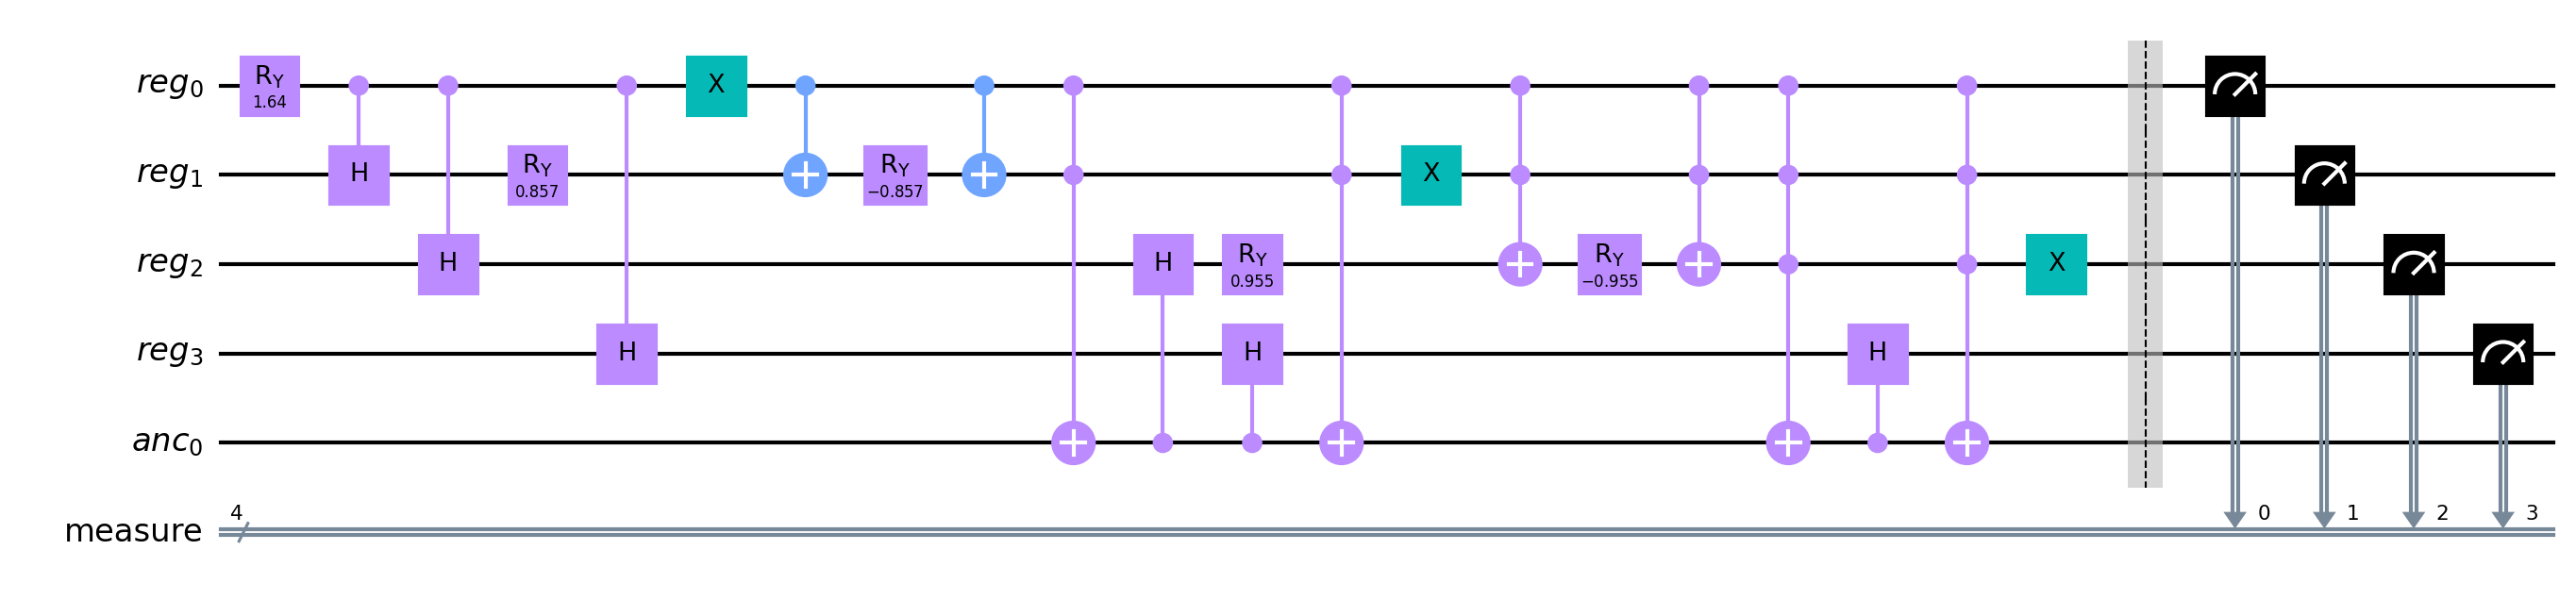
\includegraphics[width=0.8\textwidth]{images/example_circuit.png}};\\};
         \draw[marr] ([yshift=-7mm]img-1.south) coordinate (aux) 
         -- (img-2.north-|aux);
        \end{tikzpicture}
    \end{figure}
   \end{frame}
   
   \begin{frame}{Results}
       \begin{columns}
           \column{0.48\textwidth}
           \begin{center}
           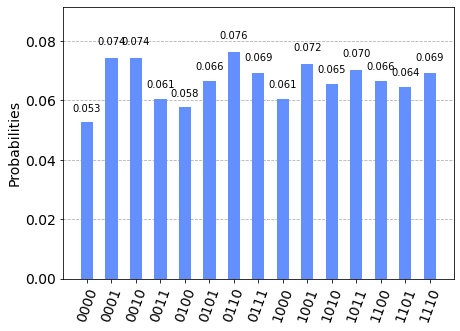
\includegraphics[width=\linewidth]{images/example_measurement.png}
           \textit{Example measurement with }\texttt{parts = 15}. \\
           \end{center}
           \textbf{Complexity} \\
           $n =$ \# elements, $o =$ \texttt{bin(n).count(`1')} \\
           Many-worlds: $O(o)$ \\
           Copenhagen: $O(o \cdot n!)$
           
           \column{0.48\textwidth}
           Gate count scales with the number of `1's in the binary representation, \textit{\textbf{not}} the size of the number.
           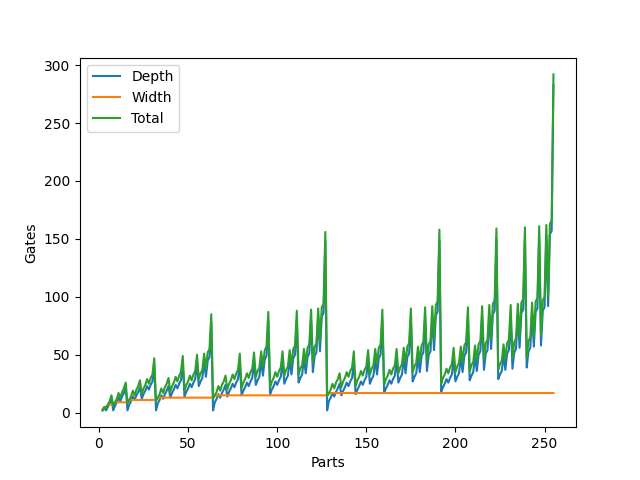
\includegraphics[width=\linewidth]{images/resources.png}
           \textit{Circuit depth, width, and total gate count in relation to} $ i $.
       \end{columns}
   \end{frame}
  
  \begin{frame}{Conclusion}
  Quantum Bogosort is not a useful algorithm, but it's helpful in teaching quantum computing fundamentals in a fun way. \\ \\
  Although infeasible due to its ballooning gate count, the QRNG algorithm could be repurposed for quickly preparing evenly balanced states among qubits. \\ \\
  By trying to optimize around the abysmal $ O(\log_2 n!) $ space complexity via `dividing and conquering', we end up implementing quicksort.
  \end{frame}
  
  \begin{frame}{Bibliography}
  \bibliographystyle{ieeetr}
  \bibliography{sources}
  \end{frame}
  
  
\end{document}